\synctex=1
\documentclass[11pt,aspectratio=169]{beamer}

\usepackage[T1]{fontenc}
\usepackage[french,provide=*]{babel}
\usepackage{amsmath,amssymb,amsfonts}
\usepackage{mathtools}
\usepackage{bm}
\usepackage{tikz}
\usetikzlibrary{arrows.meta,positioning,shapes,calc}
\usepackage{pgfplots}
\usepackage{xcolor}
\usepackage{booktabs}
\pgfplotsset{compat=1.18}

% Police serif pour les mathématiques
\usefonttheme[onlymath]{serif}

% Couleurs
\definecolor{darkblue}{RGB}{0,51,102}
\definecolor{lightblue}{RGB}{230,240,250}
\definecolor{darkgreen}{RGB}{0,102,51}
\definecolor{darkred}{RGB}{153,0,0}
\definecolor{orange}{RGB}{255,128,0}
\definecolor{violet}{RGB}{102,0,153}
\definecolor{lightgreen}{RGB}{220,245,220}
\definecolor{lightorange}{RGB}{255,240,220}
\definecolor{gray}{gray}{0.4}

% Commandes mathématiques
\newcommand{\E}{\mathbb{E}}
\newcommand{\V}{\mathbb{V}}
\newcommand{\PP}{\mathbb{P}}
\newcommand{\R}{\mathbb{R}}
\newcommand{\N}{\mathbb{N}}
\newcommand{\plim}{\overset{p}{\longrightarrow}}
\newcommand{\dlim}{\overset{d}{\longrightarrow}}
\DeclareMathOperator*{\argmax}{arg\,max}
\DeclareMathOperator*{\argmin}{arg\,min}

% Git hash
\usepackage{xstring}
\usepackage{catchfile}
\immediate\write18{git rev-parse HEAD > git.hash}
\CatchFileDef{\HEAD}{git.hash}{\endlinechar=-1}
\newcommand{\gitrevision}{\StrLeft{\HEAD}{7}}

\usepackage{ccicons}

% Pied de page personnalisé
\setbeamertemplate{footline}{
  \hfill\vspace*{1pt}\href{https://creativecommons.org/publicdomain/zero/1.0/deed.fr}{\cczero}\enspace\href{https://github.com/stepan-a/microeconometrics}{\gitrevision}\enspace--\enspace\insertframenumber/\inserttotalframenumber\enspace--\enspace\today\enspace}

% Supprimer la barre de navigation
\setbeamertemplate{navigation symbols}{}

\title{Économétrie des Variables Qualitatives}
\subtitle{Chapitre 5 : Les variables dichotomiques --- Modèles Logit et Probit}
\author{}
\date{}
\institute{}

\AtBeginSection[]
{
  \begin{frame}
    \frametitle{Plan}
    \tableofcontents[currentsection]
  \end{frame}
}

\begin{document}

\begin{frame}
\titlepage
\end{frame}

\begin{frame}{Plan}
\tableofcontents
\end{frame}

%==============================================================================
\section{Cadre général}
%==============================================================================

\begin{frame}{Cadre général -- Variable dichotomique}

\begin{itemize}

\item Une variable $y \in \{0, 1\}$ suit une \textbf{loi de Bernoulli} de
  paramètre $p$ :
  \[
  \PP(y = k) = p^k (1-p)^{1-k} = \begin{cases}
      p & \text{si } k = 1 \\
      1-p & \text{si } k = 0
  \end{cases}
  \]

\item \textbf{Espérance} : $\E[y] = 0 \times (1-p) + 1 \times p = p$.\newline

\item \textbf{Variance} : $\V[y] = p(1-p)$. Maximale pour $p = 0.5$,
  s'annule quand $p \to 0$ ou $p \to 1$.

\end{itemize}

\end{frame}

\begin{frame}{Cadre général -- Modèle conditionnel}

\begin{itemize}

\item On observe $N$ variables de Bernoulli $(y_1, \ldots, y_N)$
  \textbf{indépendantes} avec des paramètres \textbf{différents}
  $(p_1, \ldots, p_N)$.\newline

\item Les probabilités dépendent des variables explicatives $X_i$ :
  \[
  p_i = p(X_i, \beta), \quad i = 1, \ldots, N
  \]
  où $\beta$ est le paramètre à estimer.\newline

\item Contrairement au modèle marginal (statistique classique), chaque
  observation a sa propre probabilité $\Rightarrow$ modèle
  \textbf{conditionnel}.

\end{itemize}

\end{frame}

\begin{frame}{Cadre général -- Log-vraisemblance}

\begin{itemize}

\item \textbf{Log-vraisemblance} :
  \[
  \ell(y \mid X, \beta) = \sum_{i=1}^{N} \left[ y_i \ln p_i + (1-y_i) \ln(1-p_i) \right]
  \]
  où $p_i = p(X_i, \beta)$.\newline

\item \textbf{Score} :
  \[
  \frac{\partial \ell}{\partial \beta} = \sum_{i=1}^{N} \frac{\partial p_i}{\partial \beta} \cdot \frac{y_i - p_i}{p_i(1-p_i)}
  \]

\item Cette représentation est valable pour \textbf{tous} les modèles
  dichotomiques. Il suffit de spécifier la forme de $p(X_i, \beta)$.

\end{itemize}

\end{frame}

\begin{frame}{Cadre général -- Modèle latent}

\begin{itemize}

\item On suppose que la variable dichotomique observée résulte d'une variable
  \textbf{continue inobservable} $y_i^*$ :
  \[
  y_i^* = X_i \beta + u_i
  \]
  où $u_i$ est une perturbation d'espérance nulle.\newline

\item \textbf{Règle de décision} :
  \[
  y_i = \begin{cases}
      1 & \text{si } y_i^* > 0 \\
      0 & \text{si } y_i^* \leq 0
  \end{cases}
  \]

\item Le seuil 0 est conventionnel (sans incidence si le modèle contient une
  constante).

\end{itemize}

\end{frame}

\begin{frame}{Cadre général -- Probabilité}

\begin{itemize}

\item \textbf{Calcul de la probabilité} :
  \begin{align*}
      p_i &= \PP(y_i = 1) = \PP(y_i^* > 0) \\
      &= \PP(X_i \beta + u_i > 0) \\
      &= \PP(u_i > -X_i \beta) \\
      &= 1 - F(-X_i \beta)
  \end{align*}
  où $F$ est la fonction de répartition de $u_i$.\newline

\item Si $F(-z) = 1 - F(z)$ (loi symétrique), alors :
  \[
  \boxed{p_i = F(X_i \beta)}
  \]

\end{itemize}

\end{frame}

\begin{frame}{Cadre général -- Choix de la distribution}

\begin{center}
    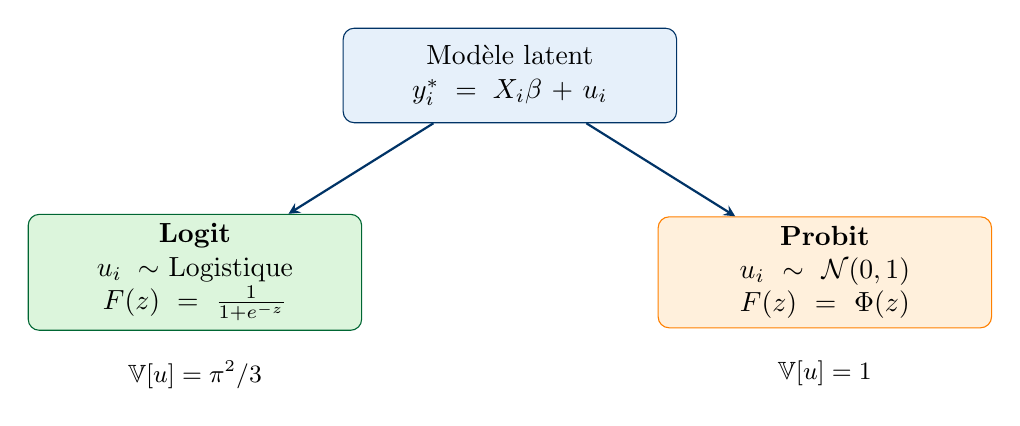
\begin{tikzpicture}[
        box/.style={rectangle, draw=darkblue, fill=lightblue, text width=4cm,
                    align=center, minimum height=1.2cm, rounded corners},
        arrow/.style={->, >=stealth, thick, darkblue}
    ]
    \node[box] (latent) at (0,0) {Modèle latent\\$y_i^* = X_i\beta + u_i$};

    \node[box, fill=lightgreen, draw=darkgreen] (logit) at (-4,-2.5)
      {\textbf{Logit}\\$u_i \sim$ Logistique\\$F(z) = \frac{1}{1+e^{-z}}$};

    \node[box, fill=lightorange, draw=orange] (probit) at (4,-2.5)
      {\textbf{Probit}\\$u_i \sim \mathcal{N}(0,1)$\\$F(z) = \Phi(z)$};

    \draw[arrow] (latent) -- (logit);
    \draw[arrow] (latent) -- (probit);

    \node[below, font=\small] at (-4,-3.5) {$\V[u] = \pi^2/3$};
    \node[below, font=\small] at (4,-3.5) {$\V[u] = 1$};
    \end{tikzpicture}
\end{center}

Les deux lois sont symétriques. Le choix entre Logit et Probit est souvent
empirique ; les résultats sont généralement similaires.

\end{frame}

%==============================================================================
\section{Le modèle Logit}
%==============================================================================

\begin{frame}{Logit -- Loi logistique}

\begin{itemize}

\item La fonction de répartition de la loi logistique standard est :
  \[
  F(z) = \frac{1}{1 + \exp(-z)} = \frac{\exp(z)}{1 + \exp(z)}
  \]

\item Propriétés :
  \begin{itemize}
  \item \textbf{Symétrie} : $F(-z) = 1 - F(z)$\newline
  \item \textbf{Densité} : $f(z) = F(z)(1 - F(z))$\newline
  \item \textbf{Moments} : $\E[u] = 0$, $\V[u] = \dfrac{\pi^2}{3} \approx 3.29$
  \end{itemize}

\item La propriété $f(z) = F(z)(1-F(z))$ simplifie considérablement les
  calculs de dérivées.

\end{itemize}

\end{frame}

\begin{frame}{Logit -- Graphique}

\begin{center}
    \begin{tikzpicture}[scale=0.8]
        \begin{scope}[shift={(-4.5,0)}]
            \draw[->] (-3,0) -- (3,0) node[right] {$z$};
            \draw[->] (0,-0.5) -- (0,3.5) node[above] {$F(z)$};
            \draw[thick, darkblue, domain=-2.8:2.8, samples=100]
              plot (\x, {3/(1+exp(-1.5*\x))});
            \draw[dashed, gray] (-3,3) -- (3,3);
            \node[left, gray] at (-3,3) {$1$};
            \node[left, gray] at (-3,1.5) {$0.5$};
            \draw[dashed, gray] (-3,1.5) -- (0,1.5);
            \node[below] at (0,-0.7) {\textbf{Répartition}};
        \end{scope}

        \begin{scope}[shift={(4.5,0)}]
            \draw[->] (-3,0) -- (3,0) node[right] {$z$};
            \draw[->] (0,-0.5) -- (0,3.5) node[above] {$f(z)$};
            \draw[thick, darkred, domain=-2.8:2.8, samples=100]
              plot (\x, {3*exp(-1.5*\x)/(1+exp(-1.5*\x))^2});
            \node[below] at (0,-0.7) {\textbf{Densité}};
        \end{scope}
    \end{tikzpicture}
\end{center}

La densité logistique ressemble à la densité normale mais avec des
\textbf{queues plus épaisses} (plus de valeurs extrêmes).

\end{frame}

\begin{frame}{Logit -- Log-vraisemblance}

\begin{itemize}

\item Avec $m_i = X_i \beta$ :
  \[
  p_i = F(m_i) = \frac{1}{1 + \exp(-m_i)}
  \]

\item \textbf{Log-vraisemblance} :
  \[
  \ell(y \mid X, \beta) = \sum_{i=1}^{N} \left[ y_i \ln F(m_i) + (1-y_i) \ln(1 - F(m_i)) \right]
  \]

\item La log-vraisemblance du Logit est \textbf{concave} $\Rightarrow$
  maximum unique, algorithmes standards convergent.

\end{itemize}

\end{frame}

\begin{frame}{Logit -- Score}

\begin{itemize}

\item En utilisant $f(m_i) = F(m_i)(1 - F(m_i))$ :
  \begin{align*}
      s(y \mid X, \beta) &= \sum_{i=1}^{N} X_i' \left[ y_i \frac{f(m_i)}{F(m_i)} - (1-y_i) \frac{f(m_i)}{1-F(m_i)} \right] \\
      &= \sum_{i=1}^{N} X_i' \left[ y_i (1-F(m_i)) - (1-y_i) F(m_i) \right]
  \end{align*}

\item \textbf{Forme simplifiée} :
  \[
  \boxed{s(y \mid X, \beta) = \sum_{i=1}^{N} X_i' (y_i - F(m_i))}
  \]

\item Le score est une somme de résidus $(y_i - p_i)$ pondérés par $X_i'$.

\end{itemize}

\end{frame}

\begin{frame}{Logit -- Hessien}

\begin{itemize}

\item \textbf{Hessien} :
  \[
  H(y \mid X, \beta) = \frac{\partial s}{\partial \beta'} = -\sum_{i=1}^{N} X_i' X_i f(m_i)
  \]
  Comme $f(m_i) > 0$ pour tout $i$, on a $H \prec 0$ (défini négatif)
  $\Rightarrow$ Newton-Raphson est \textbf{croissant}.\newline

\item \textbf{Information de Fisher} :
  \[
  I(\beta) = \E[-H \mid X, \beta] = \sum_{i=1}^{N} X_i' X_i f(m_i)
  \]

\item Le hessien ne dépend pas de $y$ $\Rightarrow$
  \textbf{Score = Newton-Raphson}.

\end{itemize}

\end{frame}

\begin{frame}{Logit -- Algorithmes}

\begin{itemize}

\item \textbf{BHHH} :
  \[
  W_{BHHH}^{-1} = -\sum_{i=1}^{N} X_i' X_i (y_i - F(m_i))^2
  \]

\item \textbf{Newton-Raphson} (= Score) :
  \[
  W_{NR}^{-1} = -\sum_{i=1}^{N} X_i' X_i f(m_i)
  \]

\item En pratique, Newton-Raphson converge très rapidement (3--5 itérations
  typiquement).

\end{itemize}

\end{frame}

%==============================================================================
\section{Le modèle Probit}
%==============================================================================

\begin{frame}{Probit -- Loi normale}

\begin{itemize}

\item La fonction de répartition de la loi normale centrée réduite est :
  \[
  F(z) = \Phi(z) = \int_{-\infty}^{z} \frac{1}{\sqrt{2\pi}} \exp\left(-\frac{s^2}{2}\right) ds
  \]

\item Propriétés :
  \begin{itemize}
  \item \textbf{Densité} : $\varphi(z) = \dfrac{1}{\sqrt{2\pi}} \exp\left(-\dfrac{z^2}{2}\right)$\newline
  \item \textbf{Dérivée} : $\varphi'(z) = -z \cdot \varphi(z)$\newline
  \item \textbf{Moments} : $\E[u] = 0$, $\V[u] = 1$
  \end{itemize}

\item La propriété $\varphi'(z) = -z \varphi(z)$ simplifie le calcul du
  hessien.

\end{itemize}

\end{frame}

\begin{frame}{Probit -- Log-vraisemblance}

\begin{itemize}

\item Avec $m_i = X_i \beta$ :
  \[
  p_i = \Phi(m_i)
  \]

\item \textbf{Log-vraisemblance} :
  \[
  \ell(y \mid X, \beta) = \sum_{i=1}^{N} \left[ y_i \ln \Phi(m_i) + (1-y_i) \ln(1 - \Phi(m_i)) \right]
  \]

\item Comme pour le Logit, la log-vraisemblance est \textbf{concave}.

\end{itemize}

\end{frame}

\begin{frame}{Probit -- Score}

\begin{itemize}

\item En notant $\varphi_i = \varphi(m_i)$ et $\Phi_i = \Phi(m_i)$ :
  \[
  s(y \mid X, \beta) = \sum_{i=1}^{N} X_i' \left[ y_i \frac{\varphi_i}{\Phi_i} - (1-y_i) \frac{\varphi_i}{1-\Phi_i} \right]
  \]

\item \textbf{Forme compacte} :
  \[
  \boxed{s(y \mid X, \beta) = \sum_{i=1}^{N} X_i' \frac{\varphi_i (y_i - \Phi_i)}{\Phi_i (1 - \Phi_i)}}
  \]

\item Contrairement au Logit, le score du Probit n'a pas de simplification
  aussi élégante.

\end{itemize}

\end{frame}

\begin{frame}{Probit -- Hessien et information de Fisher}

\begin{itemize}

\item \textbf{Hessien} :
  \[
  H = \sum_{i=1}^{N} X_i' X_i \varphi_i \left[ \frac{(y_i - \Phi_i) m_i}{\Phi_i(1-\Phi_i)} + \frac{(1-2\Phi_i)\varphi_i}{\Phi_i(1-\Phi_i)} - \frac{\varphi_i}{\Phi_i(1-\Phi_i)} \right]
  \]

\item \textbf{Information de Fisher} :
  \[
  I_1(\beta) = \E[-H \mid X, \beta] = \sum_{i=1}^{N} X_i' X_i \frac{\varphi_i^2}{\Phi_i(1-\Phi_i)}
  \]

\end{itemize}

\begin{alertblock}{Différence avec le Logit}
Le hessien \textbf{dépend de $y$} $\Rightarrow$ Score $\neq$ Newton-Raphson.
\end{alertblock}

\end{frame}

\begin{frame}{Probit -- Algorithmes}

\begin{itemize}

\item \textbf{BHHH} :
  \[
  W_{BHHH}^{-1} = -\sum_{i=1}^{N} X_i' X_i \frac{\varphi_i^2}{\Phi_i^2(1-\Phi_i)^2} (y_i - \Phi_i)^2
  \]

\item \textbf{Score} :
  \[
  W_{SC}^{-1} = -\sum_{i=1}^{N} X_i' X_i \frac{\varphi_i^2}{\Phi_i(1-\Phi_i)}
  \]

\item \textbf{Newton-Raphson} : expression complète du hessien.\newline

\item L'algorithme du Score est souvent préféré : moins de calculs que N-R,
  plus stable que BHHH.

\end{itemize}

\end{frame}

%==============================================================================
\section{Comparaison Logit / Probit}
%==============================================================================

\begin{frame}{Comparaison -- Identification}

\begin{itemize}

\item Le vrai modèle latent s'écrit :
  \[
  z_i^* = X_i b + v_i, \quad v_i \sim (0, \sigma^2)
  \]

\item On estime en fait :
  \[
  y_i^* = X_i \beta + u_i, \quad u_i \sim (0, 1)
  \]
  avec $y_i^* = z_i^*/\sigma$, $\beta = b/\sigma$ et $u_i = v_i/\sigma$.

\end{itemize}

\begin{alertblock}{Non-identification}
Les paramètres $b$ et $\sigma$ ne sont \textbf{pas identifiables séparément}. Seul $\beta = b/\sigma$ peut être estimé.
\end{alertblock}

\end{frame}

\begin{frame}{Comparaison -- Interprétation des coefficients}

\begin{itemize}

\item \textbf{Ce qu'on peut faire} :
  \begin{enumerate}
  \item Le \textbf{signe} de $\beta_j$ est le même que celui de $b_j$
    ($\sigma > 0$)\newline
  \item Le \textbf{ratio} de deux coefficients : $\beta_j/\beta_k = b_j/b_k$\newline
  \item Comparer deux écarts tirés de la \textbf{même} régression
  \end{enumerate}

\item \textbf{Ce qu'on ne peut pas faire} :
  \begin{enumerate}
  \item Comparer les coefficients de \textbf{deux régressions différentes}\newline
  \item Interpréter la \textbf{valeur absolue} d'un coefficient\newline
  \item Interpréter la \textbf{différence} entre deux coefficients
  \end{enumerate}

\end{itemize}

\end{frame}

\begin{frame}{Comparaison -- Conversion}

\begin{itemize}

\item \textbf{Probit} : $\V[u] = 1$ $\Rightarrow$
  $\beta_{\text{Probit}} = b/\sigma$.\newline

\item \textbf{Logit} : $\V[u] = \pi^2/3$ $\Rightarrow$
  $\beta_{\text{Logit}} = b/\phi$ avec
  $\phi = \sigma\sqrt{3}/\pi$.\newline

\item \textbf{Relation entre les coefficients} :
  \[
  \boxed{\beta_{\text{Probit}} \approx \frac{\sqrt{3}}{\pi} \beta_{\text{Logit}} \approx 0.55 \times \beta_{\text{Logit}}}
  \]
  \[
  \boxed{\beta_{\text{Logit}} \approx 1.81 \times \beta_{\text{Probit}}}
  \]

\item Ces conversions sont \textbf{approximatives} car la loi logistique
  n'est pas exactement normale.

\end{itemize}

\end{frame}

\begin{frame}{Comparaison -- Graphique}

\begin{center}
    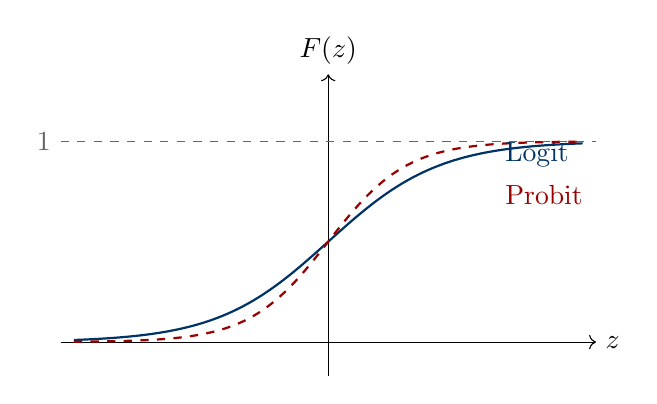
\begin{tikzpicture}[scale=0.85]
        \draw[->] (-4,0) -- (4,0) node[right] {$z$};
        \draw[->] (0,-0.5) -- (0,4) node[above] {$F(z)$};

        % Logistique
        \draw[thick, darkblue, domain=-3.8:3.8, samples=100]
          plot (\x, {3/(1+exp(-1.2*\x))});

        % Normale (approximation)
        \draw[thick, darkred, dashed, domain=-3.8:3.8, samples=100]
          plot (\x, {3/(1+exp(-1.7*\x))});

        \draw[dashed, gray] (-4,3) -- (4,3);
        \node[left, gray] at (-4,3) {$1$};

        \node[darkblue, right] at (2.5,2.8) {Logit};
        \node[darkred, right] at (2.5,2.2) {Probit};
    \end{tikzpicture}
\end{center}

Les deux courbes sont très proches. La logistique a des \textbf{queues plus
épaisses} (coefficient d'aplatissement 1.2 vs 1 pour la normale).

\end{frame}

\begin{frame}{Comparaison -- Tableau}

\begin{center}
    \small
    \renewcommand{\arraystretch}{1.3}
    \begin{tabular}{lcc}
        \toprule
        & \textbf{Logit} & \textbf{Probit} \\
        \midrule
        Distribution & Logistique & Normale \\
        Variance de $u$ & $\pi^2/3 \approx 3.29$ & $1$ \\
        Score = N-R ? & \textbf{Oui} & Non \\
        Forme fermée de $F$ & Oui & Non (intégrale) \\
        Odds ratio simple & \textbf{Oui} & Non \\
        Queues & Plus épaisses & Standard \\
        \bottomrule
    \end{tabular}
\end{center}

En pratique, le choix importe peu pour les résultats. Le Logit est souvent
préféré pour sa simplicité d'interprétation (odds ratio).

\end{frame}

%==============================================================================
\section{Aides à l'interprétation}
%==============================================================================

\begin{frame}{Interprétation -- Problème}

\begin{itemize}

\item Les coefficients $\beta$ ne sont définis qu'à une constante
  multiplicative près $\Rightarrow$ \textbf{pas directement
  interprétables}.\newline

\item Trois solutions :
  \begin{enumerate}
  \item \textbf{Odds ratio} : effet sur le rapport des probabilités\newline
  \item \textbf{Effet marginal} : $\partial p / \partial X$\newline
  \item \textbf{Effet incrémental} : variation de $p$ entre deux valeurs
    de $X$
  \end{enumerate}

\item On distingue les cas des variables explicatives \textbf{binaires} et
  \textbf{quantitatives}.

\end{itemize}

\end{frame}

\begin{frame}{Interprétation -- Odds}

\begin{itemize}

\item Pour $X \in \{0, 1\}$, les \textbf{odds} (rapport des cotes) sont :
  \[
  R(X) = \frac{\PP(Y=1 \mid X)}{\PP(Y=0 \mid X)} = \frac{F(\beta_0 + \beta_1 X)}{1 - F(\beta_0 + \beta_1 X)}
  \]

\item L'\textbf{odds ratio} mesure l'effet de $X$ :
  \[
  \psi_X = \frac{R(1)}{R(0)} = \frac{\text{odds quand } X=1}{\text{odds quand } X=0}
  \]

\item $\psi_X > 1$ signifie que $X=1$ augmente les chances de $Y=1$.

\end{itemize}

\end{frame}

\begin{frame}{Interprétation -- Odds ratio (Logit)}

\begin{itemize}

\item Pour le modèle Logit :
  \[
  R(X) = \frac{F(\beta_0 + \beta_1 X)}{1 - F(\beta_0 + \beta_1 X)} = \exp(\beta_0 + \beta_1 X)
  \]

\item \textbf{Odds ratio} :
  \[
  \boxed{\psi_X = \frac{R(1)}{R(0)} = \frac{\exp(\beta_0 + \beta_1)}{\exp(\beta_0)} = \exp(\beta_1)}
  \]

\item Il suffit de prendre l'\textbf{exponentielle du coefficient} pour
  obtenir l'odds ratio. Cette propriété est spécifique au Logit.

\end{itemize}

\end{frame}

\begin{frame}{Interprétation -- Effet incrémental}

\begin{itemize}

\item L'\textbf{effet incrémental} de $X$ sur la probabilité est :
  \[
  \Delta_X = \frac{\PP(Y=1 \mid X=1)}{\PP(Y=1 \mid X=0)} = \frac{F(\beta_0 + \beta_1)}{F(\beta_0)}
  \]

\item Pour le Logit :
  \[
  \Delta_X = \exp(\beta_1) \times \frac{1 + \exp(\beta_0)}{1 + \exp(\beta_0 + \beta_1)}
  \]

\item L'effet incrémental dépend du point de référence $\beta_0$,
  contrairement à l'odds ratio.

\end{itemize}

\end{frame}

\begin{frame}{Interprétation -- Effet marginal}

\begin{itemize}

\item L'\textbf{effet marginal} de $X$ sur la probabilité est :
  \[
  \delta_X = \frac{\partial \PP(Y=1 \mid X)}{\partial X} = \beta_1 \times f(\beta_0 + \beta_1 X)
  \]

\item L'effet marginal \textbf{varie avec $X$}. On peut :
  \begin{itemize}
  \item Évaluer au point moyen $\bar{X}$\newline
  \item Évaluer à la médiane\newline
  \item Tracer un graphique sur toutes les valeurs de $X$
  \end{itemize}

\end{itemize}

\end{frame}

\begin{frame}{Interprétation -- Effet interdécile}

\begin{itemize}

\item Mesurer la variation de probabilité quand $X$ passe du 1er décile
  ($D_1$) au 9e décile ($D_9$) :
  \[
  \Delta_{D_1 \to D_9} = F(\beta_0 + \beta_1 D_9) - F(\beta_0 + \beta_1 D_1)
  \]

\item L'effet interdécile donne une bonne idée du \textbf{potentiel
  d'influence} de $X$ sur la probabilité.\newline

\item Pour une loi normale, cela correspond à $X \pm 1.645 \sigma_X$.

\end{itemize}

\end{frame}

\begin{frame}{Interprétation -- Odds ratio quantitatif (Logit)}

\begin{itemize}

\item \textbf{Passage de $a$ à $b$} :
  \[
  \psi_X = \frac{R(b)}{R(a)} = \frac{\exp(\beta_0 + \beta_1 b)}{\exp(\beta_0 + \beta_1 a)} = \exp[\beta_1(b-a)]
  \]

\item \textbf{Cas particulier} : augmentation d'une unité ($b = a + 1$) :
  \[
  \boxed{\psi_X = \exp(\beta_1)}
  \]

\item Pour le Logit, $\exp(\beta_1)$ est l'odds ratio associé à une
  augmentation d'une unité de $X$, que $X$ soit binaire ou quantitative.

\end{itemize}

\end{frame}

%==============================================================================
\section{Application}
%==============================================================================

\begin{frame}{Application -- Données}

\begin{itemize}

\item \textbf{Données} : Enquête INSEE «~Jeunes et Carrières~» (1997),
  $N = 5425$ couples.\newline

\item \textbf{Variable expliquée} : Participation des femmes au marché du
  travail (0/1).\newline

\item \textbf{Variables explicatives} :
  \begin{itemize}
  \item Âge, nombre d'enfants, naissance récente\newline
  \item Activité des parents, nationalité\newline
  \item Niveau d'éducation (7 niveaux)\newline
  \item Région d'habitation\newline
  \item Caractéristiques du conjoint
  \end{itemize}

\end{itemize}

\end{frame}

\begin{frame}[fragile]{Application -- Syntaxe SAS}

\textbf{Estimation Logit} :
\begin{verbatim}
proc logistic data=tab descending;
    model y = x1 x2 x3;
run;
\end{verbatim}

\textbf{Estimation Probit} :
\begin{verbatim}
proc logistic data=tab descending;
    model y = x1 x2 x3 / link=normit;
run;
\end{verbatim}

L'option \texttt{descending} est \textbf{cruciale} : sans elle, SAS modélise
$\PP(Y=0)$ au lieu de $\PP(Y=1)$.

\end{frame}

\begin{frame}{Application -- Résultats}

\begin{center}
    \small
    \renewcommand{\arraystretch}{1.3}
    \begin{tabular}{lrrr}
        \toprule
        \textbf{Variable} & \textbf{Coef.} & \textbf{Écart-type} & \textbf{Significatif} \\
        \midrule
        Constante & $-0.92$ & $0.17$ & *** \\
        Âge & $+0.05$ & $0.006$ & *** \\
        1 enfant & $-0.22$ & $0.07$ & *** \\
        2 enfants & $-0.58$ & $0.07$ & *** \\
        3 enfants & $-0.98$ & $0.08$ & *** \\
        4+ enfants & $-1.61$ & $0.11$ & *** \\
        Diplôme BTS & $+1.00$ & $0.09$ & *** \\
        Diplôme Sup. & $+0.92$ & $0.10$ & *** \\
        \bottomrule
    \end{tabular}
\end{center}

Les principaux déterminants de la participation sont le \textbf{nombre
d'enfants} (effet négatif croissant) et le \textbf{niveau d'études} (effet
positif fort).

\end{frame}

%==============================================================================
\section{Récapitulatif}
%==============================================================================

\begin{frame}{Récapitulatif -- Modèle général}

\begin{center}
    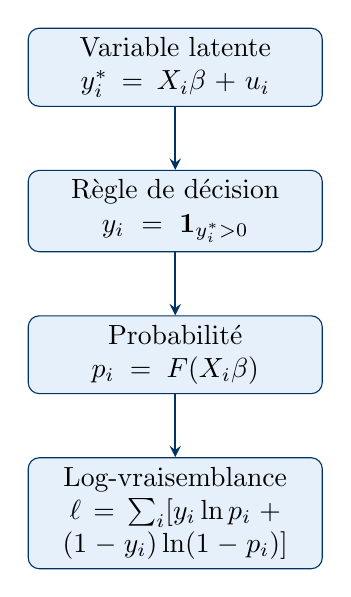
\begin{tikzpicture}[scale=0.9,
        node distance=0.8cm,
        box/.style={rectangle, draw=darkblue, fill=lightblue, text width=3.5cm,
                    align=center, minimum height=0.9cm, rounded corners},
        arrow/.style={->, >=stealth, thick, darkblue}
    ]
    \node[box] (latent) {Variable latente\\$y_i^* = X_i\beta + u_i$};
    \node[box, below=of latent] (regle) {Règle de décision\\$y_i = \mathbf{1}_{y_i^* > 0}$};
    \node[box, below=of regle] (proba) {Probabilité\\$p_i = F(X_i\beta)$};
    \node[box, below=of proba] (vrais) {Log-vraisemblance\\$\ell = \sum_i [y_i \ln p_i + (1-y_i)\ln(1-p_i)]$};

    \draw[arrow] (latent) -- (regle);
    \draw[arrow] (regle) -- (proba);
    \draw[arrow] (proba) -- (vrais);
    \end{tikzpicture}
\end{center}

\end{frame}

\begin{frame}{Récapitulatif -- Formules}

\begin{itemize}

\item \textbf{Logit} :
  \begin{align*}
      F(z) &= \frac{1}{1+e^{-z}}, \quad f(z) = F(z)(1-F(z)) \\
      s &= \sum_i X_i'(y_i - F_i), \quad H = -\sum_i X_i'X_i f_i
  \end{align*}

\item \textbf{Probit} :
  \begin{align*}
      F(z) &= \Phi(z), \quad f(z) = \varphi(z) \\
      s &= \sum_i X_i' \frac{\varphi_i(y_i - \Phi_i)}{\Phi_i(1-\Phi_i)}, \quad I = \sum_i X_i'X_i \frac{\varphi_i^2}{\Phi_i(1-\Phi_i)}
  \end{align*}

\item \textbf{Conversion} : $\beta_{\text{Probit}} \approx 0.55 \times
  \beta_{\text{Logit}}$.

\end{itemize}

\end{frame}

\begin{frame}{Récapitulatif -- Points clés}

\begin{enumerate}

\item Les modèles dichotomiques reposent sur une \textbf{variable
  latente}.\newline

\item Les coefficients ne sont identifiés qu'à \textbf{$\sigma$ près}.\newline

\item \textbf{Logit} : odds ratio simple $\exp(\beta)$,
  Score = N-R.\newline

\item \textbf{Probit} : variance normalisée à 1, trois algorithmes.\newline

\item Pour interpréter : \textbf{odds ratio}, \textbf{effet marginal},
  \textbf{effet incrémental}.\newline

\item En pratique, Logit et Probit donnent des résultats \textbf{très
  similaires}.

\end{enumerate}

\end{frame}

\begin{frame}{Récapitulatif -- Références}

\begin{itemize}

\item Greene, W. (2018). \textit{Econometric Analysis}, 8th ed., Pearson,
  ch.~17.\newline

\item Wooldridge, J. (2010). \textit{Econometric Analysis of Cross Section
  and Panel Data}, MIT Press, ch.~15.\newline

\item Train, K. (2009). \textit{Discrete Choice Methods with Simulation},
  Cambridge.\newline

\item Pour aller plus loin : chapitre 6 (variables polytomiques) et
  chapitre 7 (pseudo maximum de vraisemblance).

\end{itemize}

\end{frame}

\end{document}
